%%%%%%%%%%%%%%%%%%%%%%%%%%%%%%%%%%%%%%%%%%%%%%%%%%%%%%%%%%%%%%%%%%%%%%%%%%%%%%%%%%
\begin{frame}[fragile]\frametitle{}

\begin{center}
{\Large Language Resources and Text Pre- Processing}
\end{center}
\end{frame}

%%%%%%%%%%%%%%%%%%%%%%%%%%%%%%%%%%%%%%%%%%%%%%%%%%%%%%%%%%%%%%%%%%%%%%%%%%%%%%%%%%
\begin{frame}[fragile]\frametitle{Text Resources}
Text is available at multiple locations and in multiple formats:
\begin{itemize}
\item Web sites
\item Databases
\item Social Networks
\item MS Word and Pdf files
\item Etc. 
\end{itemize}
The collection of text is called as ``Corpora' (plural of 'Corpus').

There are often specialized APIs that let you access text from different platforms.

Not all text follows same representation (encoding) scheme.
\end{frame}


%%%%%%%%%%%%%%%%%%%%%%%%%%%%%%%%%%%%%%%%%%%%%%%%%%%%%%%%%%%%%%%%%%%%%%%%%%%%%%%%%%
\begin{frame}[fragile]\frametitle{Corpus}
\begin{center}
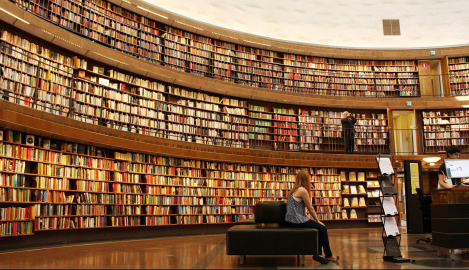
\includegraphics[width=0.7\linewidth,keepaspectratio]{corp}
\end{center}
A corpus is a collection of documents to learn about.\\
(labeled or unlabeled)
\end{frame}

%%%%%%%%%%%%%%%%%%%%%%%%%%%%%%%%%%%%%%%%%%%%%%%%%%%%%%%%%%%%%%%%%%%%%%%%%%%%%%%%%%%
%\begin{frame}[fragile]\frametitle{Pipeline}
%\begin{center}
%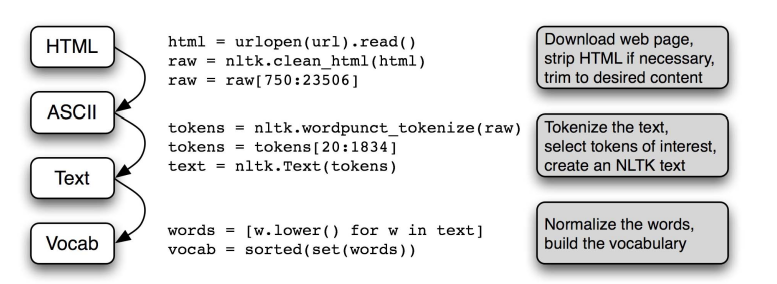
\includegraphics[width=\linewidth,keepaspectratio]{html3}
%\end{center}
%\end{frame}

%%%%%%%%%%%%%%%%%%%%%%%%%%%%%%%%%%%%%%%%%%%%%%%%%%%%%%%%%%%%%%%%%%%%%%%%%%%%%%%%%%
\begin{frame}[fragile]\frametitle{Text Encoding}

\begin{itemize}
\item ASCII is character encoding system that only supports only 128 different characters (for 7-bit encoding system or 255 for single byte):
	\begin{itemize}
	\item Sufficient for English text (128 characters are enough!!!)
	\item Insufficient for many other languages
	\item How to accommodate ALL of them?
	\end{itemize}
\item Unicode supports over a million characters:
	\begin{itemize}
	\item A single character set to cover all
	\item Each character is assigned a number, called a code point
	\item Code points are four hex numbers (\lstinline|\uXXXX|)
	\end{itemize}	
\end{itemize}
\end{frame}

%%%%%%%%%%%%%%%%%%%%%%%%%%%%%%%%%%%%%%%%%%%%%%%%%%%%%%%%%%%%%%%%%%%%%%%%%%%%%%%%%%
\begin{frame}[fragile]\frametitle{Unicode: characters are not glyphs}
\begin{itemize}
\item In Unicode, characters are abstract entities and can have more than one glyphs (written shapes)
\item A font system and additional algorithms take care after proper representation of character codes
\item UTF-8 (amongst other encodings) uses multiple bytes and can represent the full range of Unicode characters.
\end{itemize}
\end{frame}

%%%%%%%%%%%%%%%%%%%%%%%%%%%%%%%%%%%%%%%%%%%%%%%%%%%%%%%%%%%%%%%%%%%%%%%%%%%%%%%%%%%
%\begin{frame}[fragile]\frametitle{UTF-8}
%\begin{center}
%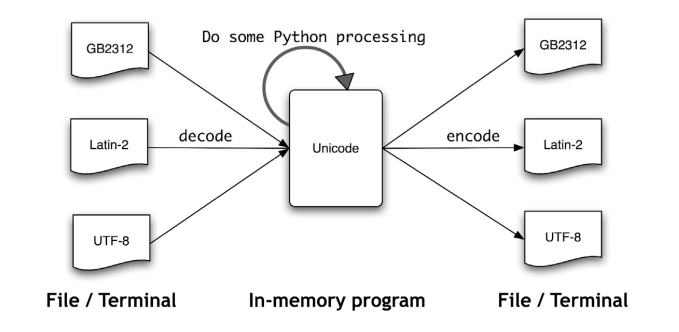
\includegraphics[width=\linewidth,keepaspectratio]{utf81}
%\end{center}
%\end{frame}

%%%%%%%%%%%%%%%%%%%%%%%%%%%%%%%%%%%%%%%%%%%%%%%%%%%%%%%%%%%%%%%%%%%%%%%%%%%%%%%%%%
\begin{frame}[fragile]\frametitle{Exercise}
\begin{itemize}
\item Create a UTF-8 file using a text editor
\item Read the file using ASCII encoding
\item Read the file using UTF-8 encoding
\item Compare the outputs
\item Convert the encoding of the file into Latin2
\lstinline|f = codecs.open(path,'w',encoding='latin2')|
\end{itemize}
\end{frame}

%%%%%%%%%%%%%%%%%%%%%%%%%%%%%%%%%%%%%%%%%%%%%%%%%%%%%%%%%%%%%%%%%%%%%%%%%%%%%%%%%%
\begin{frame}[fragile]\frametitle{Corpora}
\begin{itemize}
\item A text corpus is a large, structured collection of texts. 
\item The Open Language Archives Community (OLAC) provides an infrastructure for documenting and discovering language resource
\item OLAC is an international partnership of institutions and individuals who are creating a worldwide virtual library of language resources by: 
\begin{itemize}
\item developing consensus on best current practice for the digital archiving of language resources, and 
\item developing a network of inter-operating repositories and services for housing and accessing such resources.
\end{itemize}
\item http://www.language-archives.org/
\item NLTK comes with many corpora

\end{itemize}
\end{frame}

%%%%%%%%%%%%%%%%%%%%%%%%%%%%%%%%%%%%%%%%%%%%%%%%%%%%%%%%%%%%%%%%%%%%%%%%%%%%%%%%%%
\begin{frame}[fragile]\frametitle{Annotated Text Corpora}
\begin{itemize}
\item Many text corpora contain linguistic annotations, representing genres, POS tags, named entities, syntactic structures, semantic roles, and so forth. 
\item Not part of the text in the file; it explains something of the structure and/or semantics of text
\item Grammar annotation
\item Semantic annotation
\item Lower level annotation
\begin{itemize}
\item Word tokenization
\item Sentence Segmentation 
\item Paragraph Segmentation
\end{itemize}
\end{itemize}
\end{frame}


%%%%%%%%%%%%%%%%%%%%%%%%%%%%%%%%%%%%%%%%%%%%%%%%%%%%%%%%%%%%%%%%%%%%%%%%%%%%%%%%%%
\begin{frame}[fragile]\frametitle{Text Corpus Structure}
\begin{itemize}
\item The simplest kind lacks any structure (i.e annotation): it is just a collection of texts (Gutenberg, web text)
\item Often, texts are grouped into categories that might correspond to genre, source, author, language, etc. (Brown)
\item Sometimes these categories overlap, notably in the case of topical categories as a text can be relevant to more than one topic. (Reuters)
\item Occasionally, text collections have temporal structure (news collections, Inaugural Address Corpus)
\end{itemize}
\end{frame}


%%%%%%%%%%%%%%%%%%%%%%%%%%%%%%%%%%%%%%%%%%%%%%%%%%%%%%%%%%%%%%%%%%%%%%%%%%%%%%%%%%
\begin{frame}[fragile]\frametitle{Brown Corpus}
The Brown Corpus was the first million-word electronic corpus of English, created in 1961 at Brown University. This corpus contains text from 500 sources, and the sources have been categorized by genre, such as news, editorial, and so on. 
\begin{center}
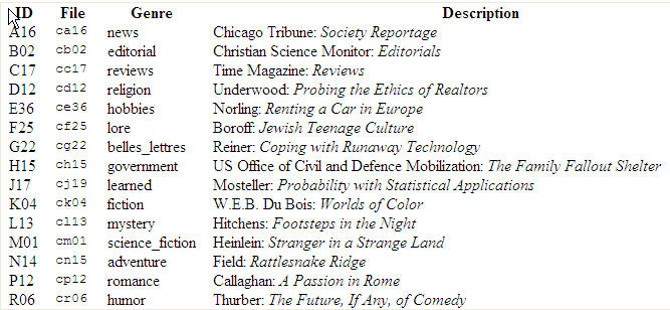
\includegraphics[width=0.8\linewidth,keepaspectratio]{corp1}
\end{center}
\end{frame}

%%%%%%%%%%%%%%%%%%%%%%%%%%%%%%%%%%%%%%%%%%%%%%%%%%%%%%%%%%%%%%%%%%%%%%%%%%%%%%%%%%
\begin{frame}[fragile]\frametitle{Brown Corpus}
\begin{itemize}
\item The Brown Corpus is a convenient resource for studying systematic differences between genres, a kind of linguistic inquiry known as stylistics.
\item For example, we can compare genres in their usage of modal verbs:
\end{itemize}
\begin{center}
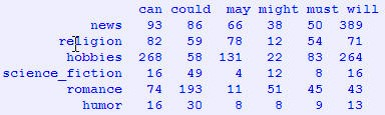
\includegraphics[width=0.6\linewidth,keepaspectratio]{corp2}
\end{center}
\end{frame}

%%%%%%%%%%%%%%%%%%%%%%%%%%%%%%%%%%%%%%%%%%%%%%%%%%%%%%%%%%%%%%%%%%%%%%%%%%%%%%%%%%
\begin{frame}[fragile]\frametitle{Reuters Corpus}
\begin{itemize}
\item The Reuters Corpus contains 10,788 news documents totaling 1.3 million words. 
\item The documents have been classified into 90 topics, and grouped into two sets, called ``training`` and ``test''
\item This split is for training and testing algorithms that automatically detect the topic of a document
\item Unlike the Brown Corpus, categories in the Reuters corpus overlap with each other, simply because a news story often covers multiple topics. 
\end{itemize}
\end{frame}

%%%%%%%%%%%%%%%%%%%%%%%%%%%%%%%%%%%%%%%%%%%%%%%%%%%%%%%%%%%%%%%%%%%%%%%%%%%%%%%%%%
\begin{frame}[fragile]\frametitle{ Lexical Resources }
\begin{itemize}
\item A lexicon, or lexical resource, is a collection of words and/or phrases along with associated information such as part of speech and sense definitions. 
\item Lexical resources are secondary to texts, and are usually created and enriched with the help of texts 
\item A vocabulary (list of words in a text) is the simplest lexical resource
\item Lexical entry
\item A lexical entry consists of a headword (also known as a lemma) along with additional information such as the part of speech and the sense definition. 
%\item Two distinct words having the same spelling are called homonyms. 
\item WordNet
\item VerbNet
\item FrameNet
%\item Medline
\end{itemize}
\end{frame}




%%%%%%%%%%%%%%%%%%%%%%%%%%%%%%%%%%%%%%%%%%%%%%%%%%%%%%%%%%%%%%%%%%%%%%%%%%%%%%%%%%
\begin{frame}[fragile]\frametitle{WordNet}
\begin{itemize}
\item WorldNet is a semantically-oriented dictionary of English, similar to a traditional thesaurus but with a richer structure.
\item WordNet is a large lexical database of English. Nouns, verbs, adjectives and adverbs are grouped into sets of cognitive synonyms (synsets), each expressing a distinct concept*. 
\item Synsets are interlinked by means of conceptual-semantic and lexical relations. The resulting network of meaningfully related words and concepts can be navigated with the browser. 
\item WordNet is also freely and publicly available for download. 
\item WordNet's structure makes it a useful tool for computational linguistics and natural language processing. 
\item NLTK includes the English WordNet, with 155,287 words and 117,659 synonym sets
\end{itemize}
\end{frame}


%%%%%%%%%%%%%%%%%%%%%%%%%%%%%%%%%%%%%%%%%%%%%%%%%%%%%%%%%%%%%%%%%%%%%%%%%%%%%%%%%%
\begin{frame}[fragile]
\frametitle{The WordNet Hierarchy}
\begin{itemize}
\item It's very easy to navigate between concepts. For example, given a concept like motorcar, we can look at the concepts that are more specific; the (immediate) hyponyms.

\begin{center}
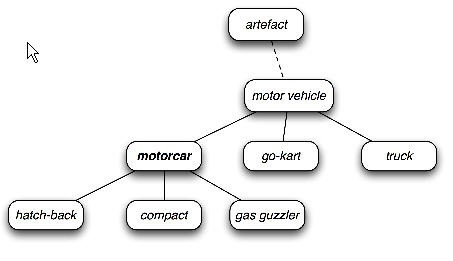
\includegraphics[width=0.8\linewidth,keepaspectratio]{word5}
\end{center}
\end{itemize}
\end{frame}

%%%%%%%%%%%%%%%%%%%%%%%%%%%%%%%%%%%%%%%%%%%%%%%%%%%%%%%%%%%%%%%%%%%%%%%%%%%%%%%%%%
\begin{frame}[fragile]
\frametitle{WordNet: Semantic Similarity}
\begin{itemize}
\item Knowing which words are semantically related is useful for indexing a collection of texts, so that a search for a general term like vehicle will match documents containing specific terms like limousine.
\item Two synsets linked to the same root may have several hypernyms in common. If two synsets share a very specific hypernym - one that is low down in the hypernym hierarchy - they must be closely related.
\end{itemize}
\end{frame}

%%%%%%%%%%%%%%%%%%%%%%%%%%%%%%%%%%%%%%%%%%%%%%%%%%%%%%%%%%%%%%%%%%%%%%%%%%%%%%%%%%
\begin{frame}[fragile]
\frametitle{VerbNet: A Verb Lexicon}
\begin{itemize}
\item VerbNet, a hierarchical verb lexicon linked to WordNet. It can be accessed with nltk.corpus.verbnet. 
\item *VerbNet is the largest on-line verb lexicon currently available for English. 
\item It is a hierarchical domain-independent, broad-coverage verb lexicon with mappings to other lexical resources such as WordNet and FrameNet.
\end{itemize}
\end{frame}


%%%%%%%%%%%%%%%%%%%%%%%%%%%%%%%%%%%%%%%%%%%%%%%%%%%%%%%%%%%%%%%%%%%%%%%%%%%%%%%%%%
\begin{frame}[fragile]
\frametitle{FrameNet}
\begin{itemize}
\item Project housed at the International Computer Science Institute (ICSI) in Berkeley, California which produces an electronic resource based on semantic frames. 	http://framenet.icsi.berkeley.edu/
\item 11,600 lexical units, in more than 960 semantic frames, exemplified in more than 150,000 annotated sentences. 
\end{itemize}
\end{frame}

%%%%%%%%%%%%%%%%%%%%%%%%%%%%%%%%%%%%%%%%%%%%%%%%%%%%%%%%%%%%%%%%%%%%%%%%%%%%%%%%%%
\begin{frame}[fragile]
\frametitle{FrameNet}
\begin{center}
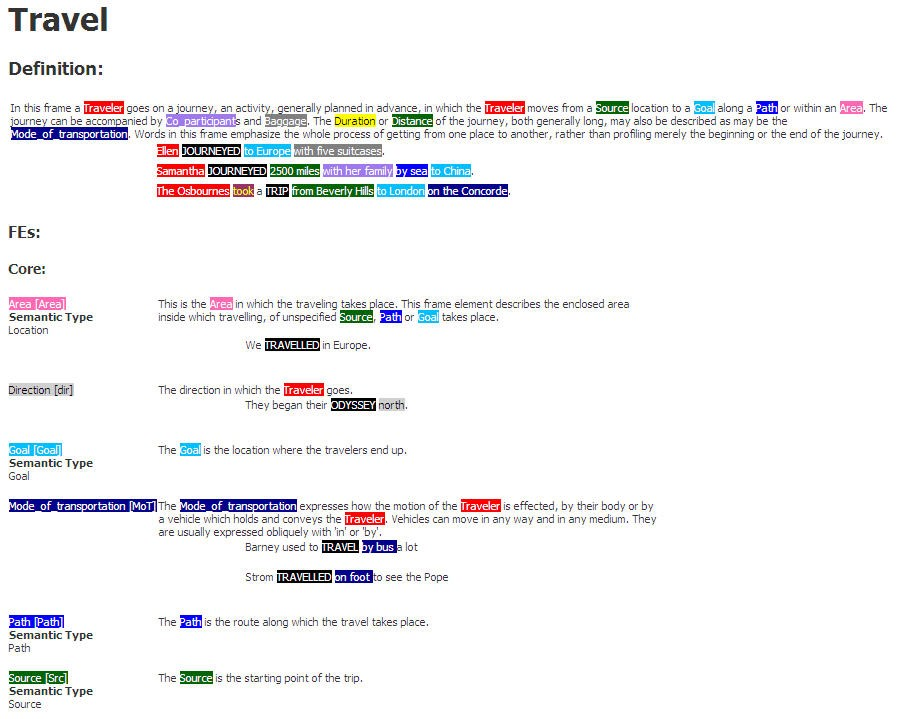
\includegraphics[width=0.7\linewidth,keepaspectratio]{word7}
\end{center}
\end{frame}

%%%%%%%%%%%%%%%%%%%%%%%%%%%%%%%%%%%%%%%%%%%%%%%%%%%%%%%%%%%%%%%%%%%%%%%%%%%%%%%%%%
\begin{frame}[fragile]
\frametitle{ Text Normalization }
\begin{itemize}
\item Stemming
\item Convert to lower case
\item Identifying non-standard words including numbers, abbreviations, and dates, and mapping any such tokens to a special vocabulary. 
\item For example, every decimal number could be mapped to a single token 0.0, and every acronym could be mapped to AAA. This keeps the vocabulary small and improves the accuracy of many language modeling tasks. 
\item Lemmatization
\item Make sure that the resulting form is a known word in a dictionary 
\item WordNet lemmatizer only removes affixes if the resulting word is in its dictionary 
\end{itemize}
\end{frame}

% %%%%%%%%%%%%%%%%%%%%%%%%%%%%%%%%%%%%%%%%%%%%%%%%%%%%%%%%%%%%%%%%%%%%%%%%%%%%%%%%%%
% \begin{frame}[fragile]
% \frametitle{Tokenization}
% \begin{itemize}
% \item Whitespace often do not indicate a word break: sometime we may want to lump together words that are separated by a white space  (whitespace?) but that we want to regard as a single word
% \item San Francisco
% \item The New York-New Heaven railroad
% \item Wake up, work out
% \end{itemize}
% \end{frame}


% %%%%%%%%%%%%%%%%%%%%%%%%%%%%%%%%%%%%%%%%%%%%%%%%%%%%%%%%%%%%%%%%%%%%%%%%%%%%%%%%%%
% \begin{frame}[fragile]
% \frametitle{ Tokenization }
% \begin{itemize}
% \item Tokenization turns out to be a far more difficult task than you might have expected. No single solution works well across-the-board, and we must decide what counts as a token depending on the application domain.
% \item When developing a tokenizer it helps to have access to raw text which has been manually tokenized, in order to compare the output of your tokenizer with high-quality (or ''gold-standard'') tokens. 
% \item The NLTK corpus collection includes a sample of Penn Treebank data, including the raw Wall Street Journal text (nltk.corpus.treebank\_raw.raw()) and the tokenized version, nltk.corpus.treebank.words()
% \end{itemize}
% \end{frame}

% %%%%%%%%%%%%%%%%%%%%%%%%%%%%%%%%%%%%%%%%%%%%%%%%%%%%%%%%%%%%%%%%%%%%%%%%%%%%%%%%%%
% \begin{frame}[fragile]
% \frametitle{ Sentence Segmentation }
% \begin{itemize}
% \item Sentence: 
% \begin{itemize}
% \item Something ending with a .. ?, ! (and sometime also :)
% \item ``You reminded me,'' she remarked, ``of your mother.''
% \begin{itemize}
% \item Nested sentences
% \item Note the .''
% \end{itemize}
% \end{itemize}
% \item Sentence boundary detection algorithms
% \begin{itemize}
% \item Heuristic (see figure 4.1 page 135 Manning)
% \item Statistical classification trees (Riley 1989)
% \item Probability of a word to occur before or after a boundary, case and length of words
% \item Neural network (Palmer and Hearst 1997)
% \item Part of speech distribution of preceding and following words
% \item Maximum Entropy (Mikheev 1998)
% \end{itemize}
% \end{itemize}
% \end{frame}

% %%%%%%%%%%%%%%%%%%%%%%%%%%%%%%%%%%%%%%%%%%%%%%%%%%%%%%%%%%%%%%%%%%%%%%%%%%%%%%%%%%
% \begin{frame}[fragile]
  % \frametitle{Stemming}
   % \begin{itemize}
  % \item The removal of the inflectional ending from words (strip off any affixes): Laughing, laugh, laughs, laughed: laugh
  % \item Problems: Can conflate semantically different words: Gallery and gall may both be stemmed to gall
  % \item A further step is to make sure that the resulting form is a known word in a dictionary, a task known as lemmatization. 
  % \end{itemize}
% \end{frame}

% %%%%%%%%%%%%%%%%%%%%%%%%%%%%%%%%%%%%%%%%%%%%%%%%%%%%%%%%%%%%%%%%%%%%%%%%%%%%%%%%%%
% \begin{frame}[fragile]
% \frametitle{ Porter Stemmer }
% \begin{itemize}
% \item Lexicon free stemmer
% \item Rewrite rules
% \begin{itemize}
% \item ATIONAL : ATE (e.g. relational, relate)
% \item FUL : $\epsilon$ (e.g. hopeful, hope)
% \item SSES: SS (e.g. caresses, caress)
% \end{itemize}
% \item Errors of Commission
% \begin{itemize}
% \item Organization: organ
% \item Policy : police
% \end{itemize}
% \item Errors of Omission
% \begin{itemize}
% \item Urgency (not stemmed to urgent)
% \item European (not stemmed to Europe)
% \end{itemize}
% \end{itemize}
% \end{frame}



% %%%%%%%%%%%%%%%%%%%%%%%%%%%%%%%%%%%%%%%%%%%%%%%%%%%%%%%%%%%%%%%%%%%%%%%%%%%%%%%%%%
% \begin{frame}[fragile]
% \frametitle{Lemmatization}
% \begin{itemize}
% \item WordNet lemmatizer only removes affixes if the resulting word is in its dictionary
% \item The WordNet lemmatizer is a good choice if you want to compile the vocabulary of some texts and want a list of valid lemmas 
% \begin{center}
% 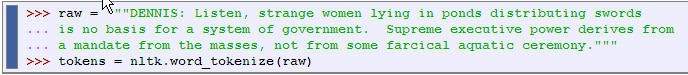
\includegraphics[width=\linewidth,keepaspectratio]{re8}
% \end{center}
% \begin{center}
% 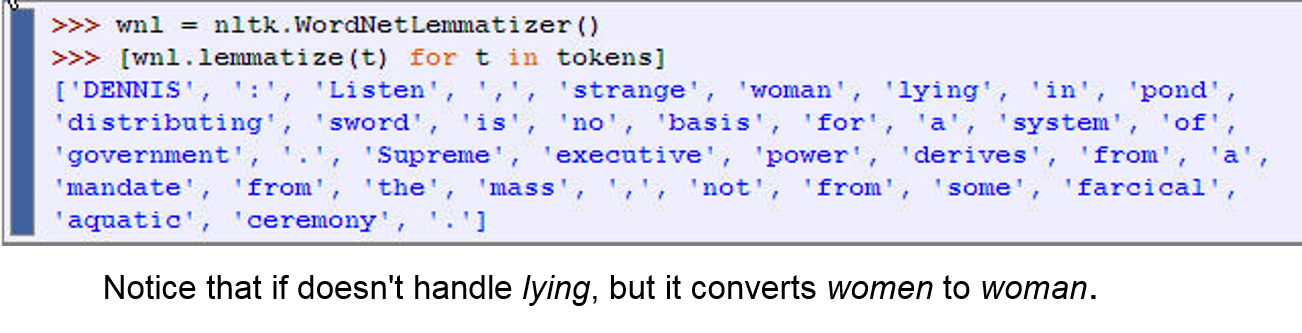
\includegraphics[width=\linewidth,keepaspectratio]{re9}
% \end{center}

% \item Notice that if doesn't handle lying, but it converts women to woman.
% \end{itemize}
% \end{frame}

% %%%%%%%%%%%%%%%%%%%%%%%%%%%%%%%%%%%%%%%%%%%%%%%%%%%%%%%%%%%%%%%%%%%%%%%%%%%%%%%%%%
% \begin{frame}[fragile]
% \frametitle{WordNet}
% \begin{itemize}
% \item We can explore these words with the help of WordNet:
% \begin{center}
% 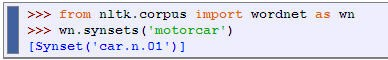
\includegraphics[width=0.8\linewidth,keepaspectratio]{word1}
% \end{center}

% \item Thus, motorcar has just one possible meaning and it is identified as car.n.01, the first noun sense of car. 
% \item The entity car.n.01 is called a synset, or ''synonym set'', a collection of synonymous words (or ''lemmas''):
% \begin{center}
% 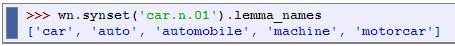
\includegraphics[width=0.9\linewidth,keepaspectratio]{word2}
% \end{center}
% \item Synsets also come with a prose definition and some example sentences: 
% \begin{center}
% 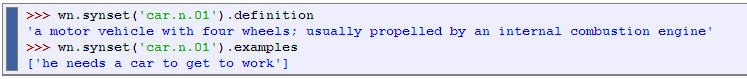
\includegraphics[width=\linewidth,keepaspectratio]{word3}
% \end{center}
% \end{itemize}
% \end{frame}

% %%%%%%%%%%%%%%%%%%%%%%%%%%%%%%%%%%%%%%%%%%%%%%%%%%%%%%%%%%%%%%%%%%%%%%%%%%%%%%%%%%
% \begin{frame}[fragile]
% \frametitle{WordNet}
% \begin{itemize}
% \item Unlike the words automobile and motorcar, which are unambiguous and have one synset, the word car is ambiguous, having five synsets:
% \begin{center}
% 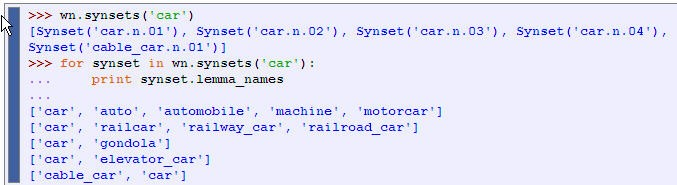
\includegraphics[width=\linewidth,keepaspectratio]{word4}
% \end{center}
% \end{itemize}
% \end{frame}

% %%%%%%%%%%%%%%%%%%%%%%%%%%%%%%%%%%%%%%%%%%%%%%%%%%%%%%%%%%%%%%%%%%%%%%%%%%%%%%%%%%
% \begin{frame}[fragile]
% \frametitle{WordNet: Semantic Similarity}
% \begin{itemize}
% \item Similarity measures have been defined over the collection of WordNet synsets which incorporate the above insight. For example, path\_similarity assigns a score in the range 0-1 based on the shortest path that connects the concepts in the hypernym 
% \begin{center}
% 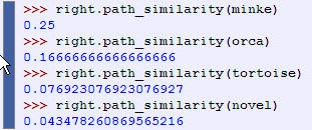
\includegraphics[width=0.5\linewidth,keepaspectratio]{word6}
% \end{center}
% \item The numbers don't mean much, but they decrease as we move away from the semantic space of sea creatures to inanimate objects. 

% \end{itemize}
% \end{frame}


%%%%%%%%%%%%%%%%%%%%%%%%%%%%%%%%%%%%%%%%%%%%%%%%%%%%%%%%%%%%%%%%%%%%%%%%%%%%%%%%%%
\begin{frame}[fragile]
\frametitle{The NLP Pipeline (Recap)}
For a given problem to be tackled:
\begin{itemize}
\item Choose corpus (or build your own)
\item Choose annotation to use (or choose the label set and label it yourself )
\item Choose or implement new NLP algorithms
\end{itemize}
\end{frame}
